\section{Definicja modelu}

\begin{frame}{MDP z dyskontowaniem quasi-hiperbolicznym}
  \begin{itemize}
    \item Model: $M = (S, A, q, r, \alpha, \beta)$.
    \item $S$ -- zbiór stanów, $A$ -- zbiór akcji.
    \item $q(s'\mid s,a)$ -- prawdopodobieństwo przejścia, $r : S \times A \rightarrow \mathbb{R}$ -- funkcja nagrody.
    \item Parametr $\alpha > 0$ wzmacnia wagę nagród natychmiastowych, $\beta \in [0,1)$ opisuje klasyczne dyskontowanie wykładnicze.
    \item Dyskontowanie quasi-hiperboliczne: $d(0) = 1$, a dla $t \ge 1$ \,$d(t) = \alpha\,\beta^t$.
  \end{itemize}
\end{frame}

\begin{frame}{Struktura interakcji agent--środowisko}
  \centering
  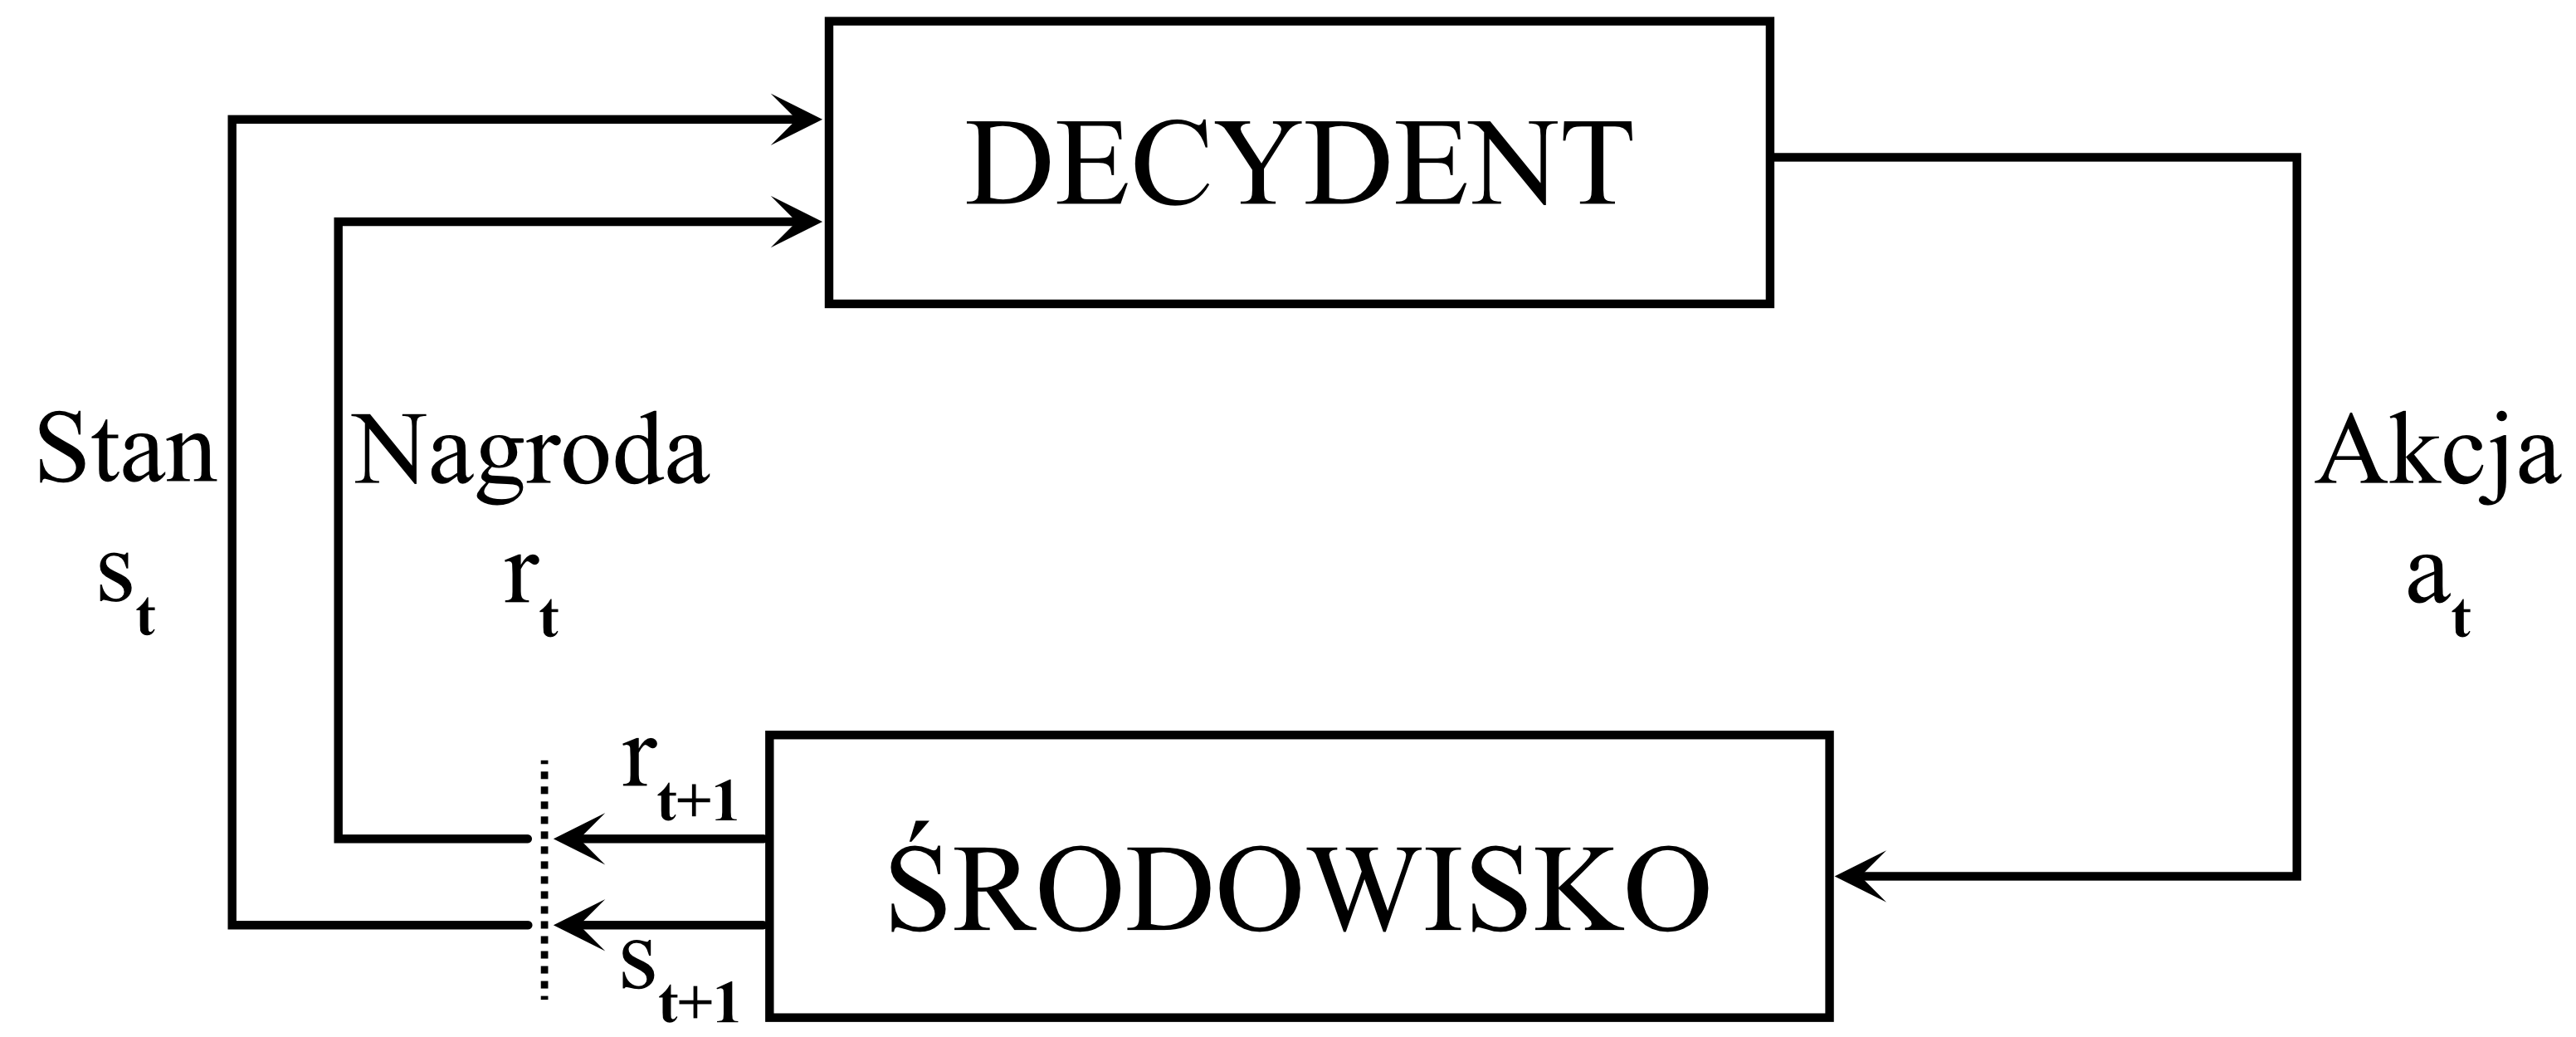
\includegraphics[width=0.9\textwidth]{../../thesis/fig/schematRL.png}
\end{frame}

\begin{frame}{Przestrzenie pomocnicze}
  \begin{itemize}
    \item $\Pr(A)$ -- zbiór miar probabilistycznych na $A$; dla skończonego $A$ utożsamiamy z $\mathbb{R}^{|A|}$.
    \item $\mathcal{H}_n$ -- historie długości $n$: $h_n = (s_0, a_0, s_1, a_1, \ldots, s_n)$, przy czym $h_0 = s_0$.
    \item Historia gromadzi pełen kontekst interakcji agent--środowisko do czasu $n$.
  \end{itemize}
\end{frame}

\begin{frame}{Polityki decyzyjne}
  Polityki decyzyjne określają rozkład akcji, które agent wybiera w danym stanie. Mamy trzy klasy polityk:
  \begin{enumerate}
    \item Ogólna polityka: $\phi = (\phi_0, \phi_1, \ldots)$, gdzie $\phi_n : \mathcal{H}_n \rightarrow \Pr(A)$.
    \item Polityki markowskie: zależne od stanu i czasu, $\phi_n : S \rightarrow \Pr(A)$.
    \item Polityki stacjonarne: zależne tylko od stanu, $\phi_s : S \rightarrow \Pr(A)$; będziemy oznaczać je przez $\phi_s$.
  \end{enumerate}
  \vspace{0.75em}
  \begin{itemize}
    \item Zbiory: $\Phi$ (wszystkie polityki), $\Phi_m$ (markowskie), $\Phi_s$ (stacjonarne).
  \end{itemize}
\end{frame}

\begin{frame}{Funkcja wypłaty}
  \small
  \begin{align}
      J_{\phi}^{\alpha,\beta}(s_0)
      &= \mathbb{E}_{\substack{a_0 \sim \phi_0(\cdot \mid s_0) \\ s' \sim q(\cdot \mid s_0,a_0)}}
        \left[ r(s_0,a_0) + \alpha\,\beta\, J_\phi^{\beta}(s') \right] = \sum_a \phi_0(a \mid s_0) \left[ r(s_0,a) + \alpha\,\beta\, \sum_{s'} P(s' \mid s_0,a) J_\phi^{\beta}(s') \right], \\
      J_\phi^{\beta}(s')
      &= \sum_{n=1}^{\infty} \beta^{n-1} \; r^{(n)}(s', \overrightarrow{\phi}).
  \end{align}
  \begin{itemize}
    \item Wagi dyskontowe: $1,\; \alpha\beta,\; \alpha\beta^2,\ldots$.
    \item $r^{(n)}$ -- oczekiwana nagroda w kroku $n$ przy polityce $\overrightarrow{\phi}$ od stanu $s'$.
  \end{itemize}
\end{frame}

\begin{frame}{oczekiwana nagroda w kroku n}
  \small
  \begin{equation*}
    r^{(n)}(s', \overrightarrow{\phi}) = \mathbb{E}_{\overrightarrow{\phi}}\!\left[ r(s_n, a_n) \;\middle|\; s_0 = s' \right].
  \end{equation*}
  \begin{itemize}
    \item Oczekiwanie po trajektoriach generowanych przez politykę $\overrightarrow{\phi} = (\phi_1, \phi_2, \ldots)$.
    \item Dla $n = 1$:
      \begin{align*}
        r^{(1)}(s_1, \overrightarrow{\phi})
        &= \sum_{a_0}\sum_{s_1}\sum_{a_1}\,
        r(s_1, a_1)\,
        \phi_1(a_1 \mid s_1,a_0,s_0)\,
          q(s_1 \mid s_0, a_0)\,
          \phi_0(a_0 \mid s_0).
      \end{align*}
    \item Dla $n = 2$:
  
    \begin{align*}
      r^{(2)}(s_2, \overrightarrow{\phi})
        &= \sum_{a_0}\sum_{s_1}\sum_{a_1}\sum_{s_2}\sum_{a_2}
          r(s_2, a_2)\,
          \phi_2(a_2 \mid s_2,a_1,s_1,a_0,s_0) \,
          q(s_2 \mid s_1, a_1)\, \\
          &\qquad{}\phi_1(a_1 \mid s_1,a_0,s_0)\,
          q(s_1 \mid s_0, a_0)\,
          \phi_0(a_0 \mid s_0).
    \end{align*}

  \end{itemize}
\end{frame}

\begin{frame}{Struktura optymalnej polityki}
  \begin{theorem}[Redukcja polityk]
    Dla dowolnej $\phi \in \Phi$ istnieją reguły $\mu$ i $\phi_s$ takie, że
    \[
      J_{\phi}^{\alpha,\beta}(s) = J_{(\mu,\phi_s)}^{\alpha,\beta}(s), \qquad \forall s \in S.
    \]
  \end{theorem}
  \begin{itemize}
    \item Pierwszy krok steruje dowolna reguła $\mu = \phi_0$, kolejne kroki wykorzystują stacjonarną $\phi_s$.
    \item Analiza optymalności sprowadza się do klas polityk dwuskładnikowych $(\mu,\phi_s)$.
  \end{itemize}
\end{frame}

\begin{frame}{Dowód redukcji polityk (1/2)}
  \small
    \textbf{Dowód.}\; Dla dowolnej historycznej polityki $\phi = (\phi_0, \phi_1, \ldots)$ mamy
  \[
    J_{\phi}^{\alpha,\beta}(s) = \mathbb{E}\!\left[ \sum_{t=0}^{\infty} d(t)\, r(s_t, a_t) \;\middle|\; s_0 = s \right],
  \]
  gdzie $d(0) = 1$ oraz $d(t) = \alpha\,\beta^{t}$ dla $t \ge 1$.
  Rozwijając wartość oczekiwaną otrzymujemy
  \[
    J_{\phi}^{\alpha,\beta}(s) = \mathbb{E}\!\left[ r(s_0,a_0) + \sum_{t=1}^{\infty} \alpha \beta^{t}\, r(s_t,a_t) \;\middle|\; s_0 = s \right].
  \]
  Warunkując po pierwszej akcji $a_0 \sim \phi_0(\cdot \mid s)$ dostajemy
  \[
    J_{\phi}^{\alpha,\beta}(s) = \mathbb{E}_{a_0 \sim \phi_0(\cdot \mid s)}\!\left[ r(s,a_0) + \,\mathbb{E}\!\left[ \sum_{t=1}^{\infty} \alpha \beta^{t}\, r(s_t,a_t) \;\middle|\; s_0 = s, a_0 \right] \right].
  \]
  Kolejne warunkowanie względem $s' \sim q(\cdot \mid s,a_0)$ daje
  \[
    J_{\phi}^{\alpha,\beta}(s) = \mathbb{E}_{\substack{a_0 \sim \phi_0(\cdot \mid s) \\ s' \sim q(\cdot \mid s,a_0)}}\!\left[ r(s,a_0) + \alpha\beta\,\mathbb{E}\!\left[ \sum_{t=1}^{\infty} \beta^{t-1}\, r(s_t,a_t) \;\middle|\; s_1=s' \right] \right].
  \]
\end{frame}

\begin{frame}{Dowód redukcji polityk (2/2)}
  \small
  Pozostała suma dyskontowana ma postać wykładniczą, więc
  \[
    \mathbb{E}\!\left[ \sum_{t=1}^{\infty} \beta^{t-1}\, r(s_t,a_t) \;\middle|\; s_1 = s' \right] = \,J_{\overrightarrow{\phi}}^{\beta}(s_1),
  \]
  gdzie $\overrightarrow{\phi} = (\phi_1, \phi_2, \ldots)$ i $J^{\beta}$ odpowiada klasycznemu dyskontowaniu wykładniczemu.
  Dla takiego dyskontowania istnieje stacjonarna polityka $\phi_s \in \Phi_s$, która spełnia
  \[
    J^{\beta}_{\overrightarrow{\phi}}(s') = J^{\beta}_{\phi_s}(s'), \qquad \forall s' \in S.
  \]
  Podstawiając do poprzedniego równania, otrzymujemy
  \[
    J_{\phi}^{\alpha,\beta}(s) = \sum_{a}\phi_{0}(a \mid s)\!\left[ r(s,a) + \alpha\,\beta\, \sum_{s'} P(s' \mid s,a) J^{\beta}_{\phi_s}(s') \right].
  \]
  Wybierając $\mu = \phi_0$ jako regułę pierwszego kroku, uzyskujemy żądaną równość
  \[
    J_{\phi}^{\alpha,\beta}(s) = J_{(\mu,\phi_s)}^{\alpha,\beta}(s), 
  \]
  co kończy dowód.
\end{frame}

